%% ICAAV 2026 -- Full-length manuscript. Springer Nature LNCS proceedings template (llncs).
%% Compile on Overleaf: set compiler to pdfLaTeX (2 passes). The reference list is an
%% inlined thebibliography block in LNCS format, numbered in order of appearance; no BibTeX run
%% is required. references.bib is included only as a convenience copy.
%% Double-blind: author names and affiliations are commented out for the initial submission.

\documentclass[runningheads]{llncs}

\usepackage{amsmath,amssymb,amsfonts}
\newcommand{\ind}{\mathbf{1}}  % indicator function (font-safe; replaces bbm's \ind)
\usepackage{graphicx}
\usepackage{xcolor}
\usepackage{booktabs}
\usepackage{multirow}
\usepackage{array}
\usepackage{url}
\usepackage{tikz}
\usetikzlibrary{positioning,arrows.meta,shapes.geometric,shapes.misc,calc,fit,backgrounds,patterns}
\usepackage[hidelinks]{hyperref}
\usepackage{microtype}
% Stop words from breaking (hyphenating) across line ends; microtype + emergencystretch
% keep the justified text tidy without those line-end hyphens.
\hyphenpenalty=10000
\exhyphenpenalty=10000
\emergencystretch=3em
\usepackage{etoolbox}
\AtBeginEnvironment{thebibliography}{\footnotesize\setlength{\itemsep}{0pt}\setlength{\parsep}{0pt}}
\setlength{\textfloatsep}{5pt plus 1pt minus 1pt}
\setlength{\intextsep}{5pt plus 1pt minus 1pt}
\setlength{\floatsep}{5pt plus 1pt minus 1pt}
\setlength{\abovecaptionskip}{3pt}
% Float-placement parameters: pack floats tighter, reduce whitespace gaps.
\renewcommand{\topfraction}{0.92}
\renewcommand{\bottomfraction}{0.85}
\renewcommand{\textfraction}{0.06}
\renewcommand{\floatpagefraction}{0.85}
\setcounter{topnumber}{3}
\setcounter{totalnumber}{4}

\begin{document}

\title{Enhancing Coverage and Localization in Multi-Altitude UAV Active SLAM Using Recurrent Proximal Policy Optimization}

%% ---- Double-blind: real author block commented out for initial submission ----
%\author{Rehaan Goenka \and Anjali Gupta \and Manish P. Singh \and Om Jee Pandey}
%\institute{Department of Electronics Engineering, Indian Institute of Technology (BHU), Varanasi, India}

\author{Anonymous Author(s)}
\institute{Anonymous Institution \\ \email{anonymous@anonymous.org}}

%% Short running heads (LNCS prints these at the top of each page; without them the
%% class substitutes "Title Suppressed Due to Excessive Length" for the long title).
\titlerunning{Multi-Altitude UAV Active SLAM with Recurrent PPO}
\authorrunning{Anonymous Author(s)}

\maketitle

%==================================================================
\begin{abstract}
Active Simultaneous Localization and Mapping (SLAM) for Unmanned Aerial Vehicles (UAVs) requires jointly maximizing map coverage and managing localization uncertainty while deciding at which altitude to fly. We propose a reinforcement learning framework that optimizes both objectives together. The proposed CoordConv--Long Short Term Memory (LSTM) recurrent Proximal Policy Optimization (PPO) actor-critic method is trained on a lightweight $48{\times}48{\times}4$ altitude grid environment. The method learns to vote horizontal displacement and altitude changes under a composite reward that combines per-step coverage gain, frontier direction progress, loop closure bonuses, altitude breadth incentives, and a novel covariance trace shaping term. Evaluated across three training seeds and fifty held out maps against six classical baselines and a Vanilla PPO learned baseline, the proposed policy delivers higher final coverage, balanced exploration of \emph{every} altitude layer, and a roughly $2{\times}$ faster time to 50\% coverage, while matching the best baseline on localization uncertainty. The headline coverage of $\mathbf{91.90 \pm 1.72\%}$ is statistically significant against every classical baseline as well as the Vanilla PPO learned baseline, and ablations on the base recipe confirm that the altitude breadth bonus stabilizes per-altitude exploration while the loop closure reward primarily reduces localization uncertainty.
\keywords{Active SLAM \and UAV exploration \and Reinforcement learning \and Recurrent PPO \and Multi-altitude planning.}
\end{abstract}

%==================================================================
\section{Introduction}

Autonomous exploration of unknown three-dimensional environments is foundational for UAVs deployed in warehouses, tunnels, disaster zones, and inspection tasks \cite{qin2019autonomous,zhang2026adaptive}. The problem is doubly coupled: the agent must move to reveal free space while localizing accurately enough to register it into a consistent global map, which is the defining concern of active SLAM~\cite{placed2023survey,zhang2026u}.

Classical active SLAM pipelines combine a frontier based or information theoretic controller with a backend SLAM estimator. These methods inherit two structural limitations: they plan on a single 2D occupancy grid, leaving altitude as a manually scheduled hyperparameter; and handcrafted cost functions struggle to jointly trade off exploration breadth, loop closure opportunity, and localization uncertainty.

Deep Reinforcement Learning (DRL) offers an attractive alternative, enabling a neural policy to learn all three concerns end-to-end. Recent work has demonstrated compelling results on 2D grids~\cite{yin2025maslam,chen2024lidar,zhao2024ddpg} and dynamic obstacle avoidance~\cite{xu2025navrl}, but altitude aware active SLAM policies remain underexplored, and the reward engineering needed to make covariance reduction trainable alongside exploration is underdocumented.

The contributions of this work are as follows:
\begin{enumerate}
    \item \textbf{Altitude as a separate decision:} 3D exploration is decomposed into horizontal movement and altitude change. Altitude is selected via a vote with a minimum dwell rule to prevent rapid layer switching, and altitude information is fed back into the observation so a single recurrent policy handles both decisions jointly.
    \item \textbf{Position-aware network with early fusion and memory:} A CoordConv led convolutional encoder encodes absolute map position, map features and SLAM scalars are combined via early fusion, and a recurrent layer carries context across the episode. This combination has not been applied to multi-altitude active SLAM before.
    \item \textbf{Reward shaping for localization:} A reward term $\Delta\sigma$ on the SLAM uncertainty surrogate $\sigma_t$ (a proxy for $\mathrm{Tr}(\Sigma_t)$) densifies the rare loop closure signal, pushing the policy toward localization improving actions. A per-altitude breadth bonus further stabilizes layer allocation, as confirmed by ablations.
    \item \textbf{Thorough evaluation:} The policy is benchmarked against six classical baselines and a Vanilla PPO baseline across multiple seeds and held out maps, achieving higher final coverage, balanced per-altitude exploration, and faster half coverage time with statistically significant gains throughout.
\end{enumerate}

%==================================================================
\section{Related Work}

Prior 3D coverage and localization work splits into classical information-theoretic active SLAM controllers and learned DRL exploration policies; we walk each thread, then surface the gap our framework closes.

\textbf{Classical active SLAM in 3D:} Placed et al.~\cite{placed2023survey} survey frontier, information-theoretic, and sampling based exploration through 2023. Asgharivaskasi and Atanasov optimize Shannon mutual information over semantic 3D octomaps~\cite{asgharivaskasi2023semantic}, extended to Riemannian multi robot optimization in~\cite{asgharivaskasi2025riemannian}. Ebadi et al.~\cite{ebadi2023extreme} and Azp\'urua et al.~\cite{azpurua2023subterranean} review 3D SLAM and autonomous exploration in extreme/subterranean environments. These methods are interpretable but plan in continuous 3D space with handcrafted costs; they neither learn a policy nor decompose altitude into discrete decisions.

\textbf{Learned 3D exploration policies:} Chen et al.~\cite{chen2024lidar} present a LiDAR based end-to-end DRL active SLAM policy; Zhao and Hwang~\cite{zhao2024ddpg} propose an exploration--exploitation DDPG variant. Botteghi et al.~\cite{botteghi2021curiosity} use curiosity driven rewards for indoor mapping; Yin et al.'s MA-SLAM~\cite{yin2025maslam} contributes a structured map representation for large scale DRL exploration on ground robots. Garaffa et al.~\cite{garaffa2023survey} survey the broader literature; Wang et al.~\cite{wang2024exploration} address exploration enhanced source search. None is altitude-aware: existing 3D capable methods operate on full continuous 3D actions or a single planar slice.

\textbf{RL for UAVs in 3D:} NavRL~\cite{xu2025navrl} trains PPO for safe 3D UAV flight with sim-to-real transfer, but targets collision free goal reaching, not mapping. Kaufmann et al.~\cite{kaufmann2023racing} surpass human champions at 3D drone racing, which is again navigation rather than exploration. Ni et al.~\cite{ni2022recurrent} establish recurrent model-free RL as a strong Partially Observable Markov Decision Process (POMDP) baseline (motivating our LSTM backbone); Raffin et al.~\cite{raffin2021sb3} provide the Stable-Baselines3 Recurrent PPO used here.

%==================================================================
\section{System Model and Problem Formulation}

\subsection{System Model}
Fig.~\ref{fig:sysmodel} depicts the closed loop system for autonomous warehouse inspection. The full 3D planning problem is decomposed into \emph{(i)} horizontal navigation within a fixed altitude layer and \emph{(ii)} discrete altitude selection, with a single recurrent policy arbitrating between the two.

\textbf{UAV and environment:} A quadrotor carries a 2D LiDAR scanner performing a $360^\circ$ sweep with $N_r\!=\!36$ beams at the current altitude, plus a half-range sweep on each adjacent layer to emulate inter-layer sensor bleed. LiDAR is preferred for its illumination robustness and native compatibility with occupancy mapping. The warehouse is partitioned into four altitude layers $h_{\text{alt}}\!\in\!\{1,2,3,4\}\,\text{m}$ over an $X\!\times\!Y$ grid; the unknown true occupancy is a binary tensor $\mathcal{M}^{\star}\!\in\!\{0,1\}^{X\times Y\times 4}$ to be reconstructed within a fixed episode budget.

\textbf{Perception and observation:} The full sweep $\{r_{i,t}\}_{i=1}^{N_r}$ is fused by an RTAB-Map inspired SLAM proxy maintaining an occupancy estimate $\mathcal{M}_t$, pose estimate $\hat{\xi}_t$, and uncertainty surrogate $\sigma_t\!\in\![0,4]$ (proxy for $\mathrm{Tr}(\Sigma_t)$), updated as $\sigma_{t+1}\!=\!\min(\sigma_t + 0.03\,\|\Delta p_t\| + 0.15\,\ind[\text{alt change}],\,4)$ and multiplied by $0.70$ on loop closure. This is compressed into $o_t\!=\!(M_t,v_t)$: the map tensor $M_t\!\in\![0,1]^{5\times 48\times 48}$ stacks five altitude-aware channels (current altitude occupancy; binary visit mask; trajectory trail; least explored altitude occupancy; cross altitude mean visit mask), and $v_t\!\in\![0,1]^{10}$ encodes normalized uncertainty, frontier count, coverage, frontier distance and direction, altitude index, per-altitude coverage statistics, and step fraction $t/T_{\max}$.

\textbf{Policy and control loop:} The recurrent policy $\pi_\theta(a_t\!\mid\!o_t,h_t)$, parameterized by $\theta$ with recurrent hidden state $h_t$ (LSTM state, defined in Section~\ref{sec:arch}), emits a continuous action $a_t\!=\!(dx_t,dy_t,dz_t)\!\in\![-1,1]^3$: the first two components drive a clipped horizontal velocity command; $dz_t$ is an altitude \emph{vote} that triggers a layer change only when $|dz_t|\!>\!\tau_{\text{alt}}$, where $\tau_{\text{alt}}\!=\!0.3$ is the altitude vote threshold, and is further gated by a minimum dwell of $D\!=\!20$ steps since the last layer change, preventing the policy from thrashing the mapping backend's Z-filter.

\begin{figure}[tb]
\centering
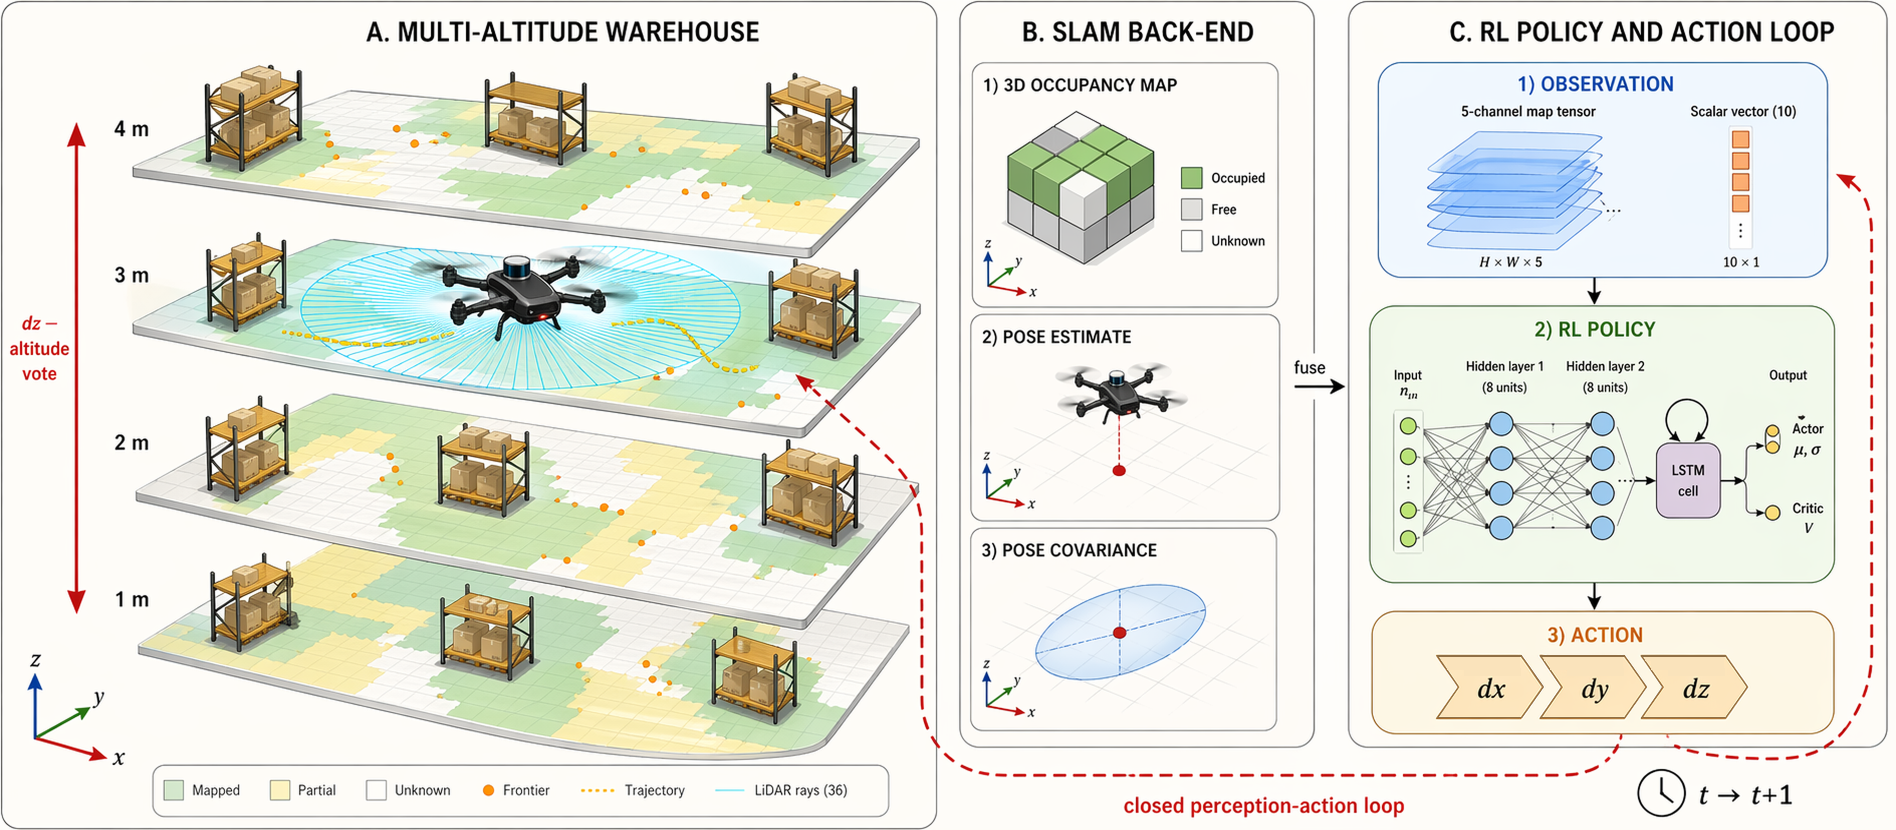
\includegraphics[width=0.86\textwidth,height=0.28\textwidth,keepaspectratio]{figures/Group 8.png}
\caption{System model: 2D LiDAR feeds a SLAM back-end producing observation $o_t$ for the RL policy, which emits action $a_t$.}
\label{fig:sysmodel}
\end{figure}

\subsection{Problem Formulation}
\vspace{-2pt}
We cast the task as a POMDP $\mathcal{P}\!=\!\langle\mathcal{S},\mathcal{A},\mathcal{O},T,O_{\text{obs}},R,\gamma,T_{\max}\rangle$ over state, action, and observation spaces, with transition kernel $T$, observation kernel $O_{\text{obs}}$, reward $R$, discount $\gamma$, and horizon $T_{\max}$. The hidden state bundles the (true, unhatted) UAV pose, occupancy $\mathcal{M}_t$, and the scalar uncertainty surrogate $\sigma_t$ from the System Model, namely $s_t = (x_t, y_t, z_t, \mathcal{M}_t, \sigma_t) \in \mathcal{S}$, with $\mathcal{A}\!=\![-1,1]^3$ and $\mathcal{O}\!=\![0,1]^{5\times 48\times 48}\!\times\![0,1]^{10}$ inheriting the dimensions of $a_t$ and $o_t\!=\!(M_t,v_t)$ from the System Model; $O_{\text{obs}}(\cdot|s_t)$ realizes the SLAM to observation compression, and $T(\cdot|s_t,a_t)$ is driven by UAV kinematics, SLAM updates, and loop closure events. Heading $\psi_t$ is not stored: it is implicit in the velocity command and recomputed on demand from $(p_t-p_{t-1})$ when needed for the relative frontier direction scalar.

\noindent\textbf{Objective as a function of $\theta$:} Let $\pi_\theta\!:\!\mathcal{O}\!\times\!\mathcal{H}\!\to\!\Delta(\mathcal{A})$ be the recurrent policy parameterized by $\theta$, with hidden state space $\mathcal{H}$ (the LSTM state of Section~\ref{sec:arch}) and $\Delta(\mathcal{A})$ the simplex of distributions over $\mathcal{A}$; let $\tau\!=\!(s_0,o_0,a_0,\ldots,s_{T_{\max}})$ be a trajectory it induces on $\mathcal{P}$. The \emph{expected discounted return} is
\vspace{-2pt}
\begin{equation}
J(\theta) \,=\, \mathbb{E}_{\tau\sim\pi_\theta}\!\left[\,\sum_{t=0}^{T_{\max}-1}\gamma^{\,t}\, R(s_t,a_t)\,\right],
\label{eq:J}
\end{equation}
\vspace{-4pt}

\noindent with $R$ the composite reward of Section~\ref{sec:reward}; $\gamma\!=\!0.995$ gives an effective horizon $1/(1-\gamma)\!\approx\!200$ steps, matched to the $T_{\max}\!=\!600$-step budget of the headline recipe ($\sim$150 steps per altitude over four layers). The target is $\theta^{\star} = \arg\max_{\theta} J(\theta)$ with $\pi^{\star} = \pi_{\theta^{\star}}$, subject to the constraint set
\vspace{-4pt}
{\renewcommand{\arraystretch}{0.80}%
\begin{equation}
\mathcal{C}:\
\begin{cases}
a_t \in [-1,1]^3, & \forall\, t \\
a_t \sim \pi_\theta(\cdot\!\mid\!o_t,h_t), & \forall\, t \\
s_{t+1} \sim T(\cdot\!\mid\!s_t,a_t), & \forall\, t \\
o_t \sim O_{\text{obs}}(\cdot\!\mid\!s_t), & \forall\, t \\
\mathrm{alt}(t) \in \{0,1,2,3\}, & \forall\, t \\
t - \tau_{\text{last}}(t) \geq D = 20, & \text{if alt.\ change at } t \\
(x_t, y_t, z_t) \in \mathcal{F}, & \forall\, t \\
0 \leq t < T_{\max}, & T_{\max}\!\in\!\{400,600\} \\
\mathrm{Cov}(s_t)\!\geq\!0.95 \Rightarrow \text{terminate}, &
\end{cases}
\label{eq:constraints}
\end{equation}}%
\vspace{-4pt}

\noindent where $\mathrm{alt}(t)\!=\!\lfloor z_t\rfloor\!-\!1\!\in\!\{0,1,2,3\}$ indexes the four altitude layers (recall $z_t\!\in\!\{1,2,3,4\}\,\text{m}$), $\mathcal{F}$ is collision free configuration space, $\tau_{\text{last}}(t)$ is the most recent altitude change timestep, and $D\!=\!20$ is the dwell from the System Model (set to suppress Z-filter thrashing). For ablation variants and the base/Vanilla recipes the horizon is $T_{\max}\!=\!400$; only the final headline ``MS600'' recipe uses $T_{\max}\!=\!600$.

\noindent\textbf{Coverage--localization trade-off:} Let $\mathrm{Cov}(s)$ be the fraction of true free cells in $\mathcal{M}^{\star}$ that have been observed by state $s$, and define $\mathcal{K}(\theta)\!:=\!\mathbb{E}_{\tau\sim\pi_\theta}[\mathrm{Cov}(s_{T_{\max}})]$, $\mathcal{U}(\theta)\!:=\!\mathbb{E}_{\tau\sim\pi_\theta}[\sigma_{T_{\max}}]$. Equation~\eqref{eq:J} then admits the scalarized form $J(\theta) = \mathcal{K}(\theta) - \lambda_\sigma\,\mathcal{U}(\theta) + \Psi(\theta)$ (coverage maximization, uncertainty minimization, and shaping, respectively), with $\lambda_\sigma\!>\!0$ realized implicitly through the reward weights and $\Psi(\theta)$ collecting the per-step shaping terms (new cell, frontier, loop closure, breadth, absolute $\sigma$ penalty, and $\Delta\sigma$) of Section~\ref{sec:reward}.

%==================================================================
\section{Proposed Methodology}\label{sec:arch}

The policy $\pi_\theta$ is a CoordConv--LSTM actor-critic trained with Recurrent PPO~\cite{raffin2021sb3,ni2022recurrent}. It is shaped by three task specific requirements: \emph{(i)} the filters must exploit absolute spatial position on the altitude grid; \emph{(ii)} the spatial map tensor and the scalar feature vector must be fused \emph{before} the policy commits to an action; and \emph{(iii)} partial observability demands memory across the $600$-step episode. Fig.~\ref{fig:arch} shows the complete network.

\begin{figure}[tb]
\centering
\resizebox{0.9\textwidth}{!}{
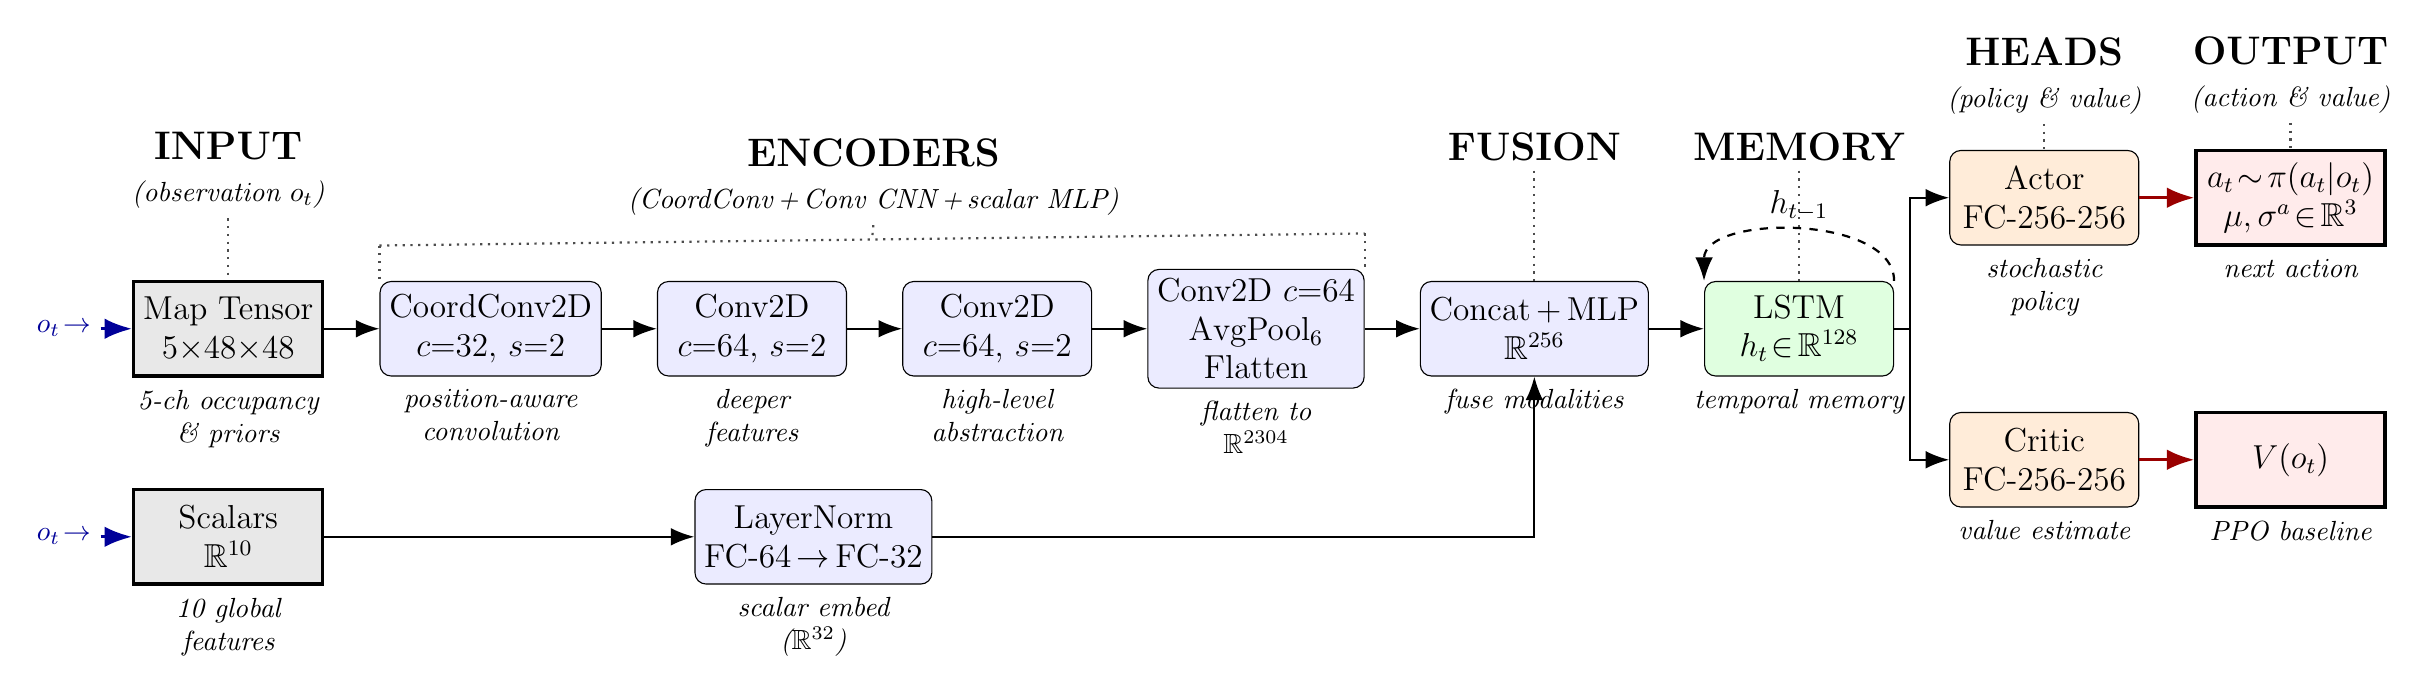
\begin{tikzpicture}[
    font=\large,
    block/.style={rectangle, draw, rounded corners, minimum height=1.2cm, minimum width=2.4cm, align=center, fill=blue!8, text=black},
    inbox/.style={rectangle, draw, very thick, minimum height=1.2cm, minimum width=2.4cm, align=center, fill=gray!18, text=black},
    outbox/.style={rectangle, draw, very thick, minimum height=1.2cm, minimum width=2.4cm, align=center, fill=red!8, text=black},
    head/.style={rectangle, draw, rounded corners, minimum height=1.2cm, minimum width=2.4cm, align=center, fill=orange!15, text=black},
    lstm/.style={rectangle, draw, rounded corners, minimum height=1.2cm, minimum width=2.4cm, align=center, fill=green!12, text=black},
    stage/.style={font=\Large\bfseries, text=black, align=center},
    sub/.style={font=\normalsize\itshape, text=black, align=center},
    ann/.style={font=\normalsize\itshape, text=black, align=center, inner sep=1pt},
    arr/.style={-{Latex[length=3mm]}, thick, text=black},
    startarr/.style={-{Latex[length=3.5mm]}, very thick, color=blue!60!black},
    endarr/.style={-{Latex[length=3.5mm]}, very thick, color=red!60!black},
    grouparr/.style={dotted, thick, color=black!70},
    node distance=0.65cm and 0.70cm
]
% ============================================================
% BLOCKS — defined first so headers can position relative to them
% ============================================================
\node[inbox] (map) {Map Tensor\\$5{\times}48{\times}48$};
\node[inbox, below=1.4cm of map] (scalars) {Scalars\\$\mathbb{R}^{10}$};

\node[left=0.4cm of map,  font=\normalsize\bfseries, color=blue!60!black] (inlab1) {$o_t\!\to$};
\node[left=0.4cm of scalars, font=\normalsize\bfseries, color=blue!60!black] (inlab2) {$o_t\!\to$};

\node[block, right=of map]   (cc1)  {CoordConv2D\\$c{=}32,\,s{=}2$};
\node[block, right=of cc1]   (cc2)  {Conv2D\\$c{=}64,\,s{=}2$};
\node[block, right=of cc2]   (cc3)  {Conv2D\\$c{=}64,\,s{=}2$};
\node[block, right=of cc3]   (fc256){Conv2D $c{=}64$\\AvgPool$_{6}$\\Flatten};

\node[block, right=4.7cm of scalars] (mlp) {LayerNorm\\FC-64\,$\to$\,FC-32};

\node[block, right=of fc256] (concat) {Concat\,+\,MLP\\$\mathbb{R}^{256}$};
\node[lstm,  right=of concat] (lstm)  {LSTM\\$h_t\!\in\!\mathbb{R}^{128}$};

\node[head,   above right=0.45cm and 0.7cm of lstm] (actor)  {Actor\\FC-256-256};
\node[head,   below right=0.45cm and 0.7cm of lstm] (critic) {Critic\\FC-256-256};

\node[outbox, right=of actor]  (action) {$a_t\!\sim\!\pi(a_t|o_t)$\\$\mu,\sigma^{a}\!\in\!\mathbb{R}^3$};
\node[outbox, right=of critic] (value)  {$V(o_t)$};

\node[ann, below=0.12cm of map]     {5-ch occupancy\\\& priors};
\node[ann, below=0.12cm of scalars] {10 global\\features};
\node[ann, below=0.12cm of cc1]     {position-aware\\convolution};
\node[ann, below=0.12cm of cc2]     {deeper\\features};
\node[ann, below=0.12cm of cc3]     {high-level\\abstraction};
\node[ann, below=0.12cm of fc256]   {flatten to\\$\mathbb{R}^{2304}$};
\node[ann, below=0.12cm of mlp]     {scalar embed\\($\mathbb{R}^{32}$)};
\node[ann, below=0.12cm of concat]  {fuse modalities};
\node[ann, below=0.12cm of lstm]    {temporal memory};
\node[ann, below=0.12cm of actor]   {stochastic\\policy};
\node[ann, below=0.12cm of critic]  {value estimate};
\node[ann, below=0.12cm of action]  {next action};
\node[ann, below=0.12cm of value]   {PPO baseline};

\node[stage, above=1.4cm of map]    (h_in)  {INPUT};
\node[sub,   below=0.02cm of h_in]  (h_in_sub)   {(observation $o_t$)};

\node[stage] (h_enc) at ($(cc1.north)!0.5!(fc256.north) + (0, 1.55)$) {ENCODERS};
\node[sub,   below=0.02cm of h_enc] (h_enc_sub) {(CoordConv\,+\,Conv CNN\,+\,scalar MLP)};

\node[stage, above=1.4cm of concat] (h_fus) {FUSION};
\node[stage, above=1.4cm of lstm]   (h_mem) {MEMORY};

\node[stage, above=0.95cm of actor] (h_head) {HEADS};
\node[sub,   below=0.02cm of h_head] (h_head_sub) {(policy \& value)};

\node[stage, above=0.95cm of action] (h_out) {OUTPUT};
\node[sub,   below=0.02cm of h_out]  (h_out_sub)  {(action \& value)};

\draw[startarr] (inlab1.east) -- (map.west);
\draw[startarr] (inlab2.east) -- (scalars.west);
\draw[arr] (map) -- (cc1);
\draw[arr] (cc1) -- (cc2);
\draw[arr] (cc2) -- (cc3);
\draw[arr] (cc3) -- (fc256);
\draw[arr] (scalars) -- (mlp);
\draw[arr] (fc256) -- (concat);
\draw[arr] (mlp.east) -- ([xshift=2mm]mlp.east) -| (concat.south);
\draw[arr] (concat) -- (lstm);
\draw[arr] (lstm.east) -- ([xshift=2mm]lstm.east) |- (actor.west);
\draw[arr] (lstm.east) -- ([xshift=2mm]lstm.east) |- (critic.west);
\draw[endarr] (actor)  -- (action);
\draw[endarr] (critic) -- (value);

\draw[arr, dashed] (lstm.north east) to[out=90, in=90, looseness=0.9]
    node[above, midway, font=\large]{$h_{t-1}$} (lstm.north west);

\draw[grouparr] (h_in_sub.south) -- (map.north);

\coordinate (encL) at ($(cc1.north west)  + (0, 0.45)$);
\coordinate (encR) at ($(fc256.north east) + (0, 0.45)$);
\coordinate (encM) at ($(encL)!0.5!(encR)$);
\draw[grouparr] (encL) -- (encR);
\draw[grouparr] (encL) -- (cc1.north west);
\draw[grouparr] (encR) -- (fc256.north east);
\draw[grouparr] (h_enc_sub.south) -- (encM);

\draw[grouparr] (h_fus.south) -- (concat.north);
\draw[grouparr] (h_mem.south) -- (lstm.north);
\draw[grouparr] (h_head_sub.south) -- (actor.north);
\draw[grouparr] (h_out_sub.south) -- (action.north);

\end{tikzpicture}
}
\caption{Proposed CoordConv--LSTM actor-critic. Map tensor is encoded by one CoordConv and three Conv2D stages; scalars by an MLP. Early fused $256$-D embedding feeds a single layer LSTM (hidden state $h_t$, dashed self-loop), then two $(256,256)$ heads output the action distribution and state value.}
\label{fig:arch}
\end{figure}

\subsection{Network Design}

\textbf{Spatial map encoder:} Starting from the five altitude aware channels of $M_t\!\in\![0,1]^{5{\times}48{\times}48}$ (current altitude occupancy, current altitude binary visit mask, exponentially decaying trajectory, least explored altitude occupancy as a soft exploration prior, and cross altitude mean visit mask), one CoordConv (kernel $5$, stride $2$) and three plain Conv2D stages (two stride-$2$ followed by one stride-$1$, all kernel $3$) compute
\begin{equation}
F^{(\ell)}_t \,=\, \sigma\big(\mathrm{GN}_8\big(W^{(\ell)}\!*\!\widetilde{F}^{(\ell-1)}_t + b^{(\ell)}\big)\big),
\label{eq:coordconv}
\end{equation}
with $F^{(0)}_t\!=\!M_t$, weights $W^{(\ell)}$ and biases $b^{(\ell)}$, channel widths $32\!\to\!64\!\to\!64\!\to\!64$ across the four stages, $\sigma(\cdot)$ the ReLU, and $\mathrm{GN}_8$ a GroupNorm with $8$ groups. Only the first stage is coordinate augmented: $\widetilde{F}^{(0)}_t$ stacks $M_t$ with two normalized coordinate maps $(i/H,\,j/W)$ over feature map indices $(i,j)$ of height $H$ and width $W$; for $\ell\!\geq\!1$, $\widetilde{F}^{(\ell-1)}_t\!=\!F^{(\ell-1)}_t$. These coordinate channels give filters direct access to \emph{absolute} position, a property plain convolutions lack and one that matters in active SLAM, where the same local pattern has different navigational value at a map's centre than at its boundary. The three strided stages collapse the $48{\times}48$ input through $24{\times}24\!\to\!12{\times}12\!\to\!6{\times}6$; the fourth (stride-$1$) stage refines features at $6{\times}6$, and an adaptive $6{\times}6$ average pool $\mathrm{AvgPool}_{6}$ (acting as identity here) followed by flattening yields the map feature $z^{\text{map}}_t = \mathrm{vec}(\mathrm{AvgPool}_{6}(F^{(4)}_t)) \in \mathbb{R}^{2304}$.

\textbf{Scalar encoder and early fusion:} The vector $v_t\!\in\![0,1]^{10}$ (normalized covariance trace, frontier statistics, per-altitude coverages, episode progress) is layer normalized and passed through a two layer MLP $g_{\psi_v}$ with parameters $\psi_v$, giving $z^{\text{scl}}_t\!=\!g_{\psi_v}(v_t)\!\in\!\mathbb{R}^{32}$. The map and scalar embeddings are concatenated and reprojected by a two layer fusion MLP $g_{\psi_f}$ with parameters $\psi_f$, giving $z_t = g_{\psi_f}([z^{\text{map}}_t; z^{\text{scl}}_t]) \in \mathbb{R}^{256}$. This \emph{early} fusion is deliberate: the policy must reason over spatial layout and scalar state jointly (``move toward this frontier \emph{because} covariance is high''), whereas late fusion would force the branches to commit to independent sub-decisions before merging.

\textbf{Recurrent backbone:} A single layer LSTM with hidden size $128$ and parameters $\phi$ propagates context across the episode, $(h_t,c_t) = \mathrm{LSTM}_{\phi}(z_t; h_{t-1}, c_{t-1})$ with $h_t,c_t\!\in\!\mathbb{R}^{128}$, where $h_t$ is the hidden state, $c_t$ the cell state, and $(h_0,c_0)\!=\!\mathbf{0}$ at episode start. Recurrence is indispensable: the observation is a lossy compression of history (the trajectory channel fades old visits, and $v_t$ squeezes the SLAM state into ten numbers), so $h_t$ must carry intent across multi-step strategies (e.g.\ ``commit to altitude 3 for 40 steps'') that no Markovian head could express.

\textbf{Actor and critic heads:} Two independent $(256,256)$ MLPs $f_{\theta_\pi}, f_{\theta_V}$ with parameters $\theta_\pi, \theta_V$ branch from $h_t$. The actor parameterizes a diagonal Gaussian over $\mathbb{R}^3$ with mean $\mu_t\!\in\!\mathbb{R}^3$ and log standard deviation $\log\sigma^{a}_t\!\in\!\mathbb{R}^3$: $(\mu_t,\log\sigma^{a}_t) = f_{\theta_\pi}(h_t)$ and $a_t \sim \mathcal{N}(\mu_t,\mathrm{diag}((\sigma^{a}_t)^2))$, where the action standard deviation $\sigma^{a}_t$ is distinct from the uncertainty surrogate $\sigma_t$; the critic outputs a scalar state value $V_{\theta_V}(o_t)\!=\!f_{\theta_V}(h_t)$. Training minimizes the joint objective
\begin{equation}
\mathcal{L}(\theta_\pi,\theta_V) \,=\, \mathcal{L}^{\text{CLIP}}(\theta_\pi) \,+\, c_1\,\big(V_{\theta_V}(o_t)\!-\!\hat{R}_t\big)^2 \,-\, c_2\,\mathcal{H}[\pi_{\theta_\pi}],
\label{eq:ppo_loss}
\end{equation}
where $\mathcal{L}^{\text{CLIP}}$ is PPO's clipped surrogate objective, $\hat{R}_t$ is the Generalized Advantage Estimation (GAE) target, $\mathcal{H}[\pi_{\theta_\pi}]$ an action-entropy bonus, and $c_1,c_2\!>\!0$ are scalar weighting coefficients~\cite{raffin2021sb3}. Separate actor/critic parameters let the critic fit the higher-frequency value signal without destabilizing the actor.

\subsection{Reward Design}\label{sec:reward}
The per-step reward $r_t$ is a weighted sum of fifteen components (Table~\ref{tab:reward}):
\begin{multline}
    r_t = w_{\Delta n}\,\Delta n_{\text{cell}} + w_{\Delta d}\,\Delta d_{\text{front}} + w_\sigma\,(\sigma_t/4) \\
    + w_{\Delta\sigma}\,\Delta\sigma + w_{\text{alt}}\,\ind[\text{new alt}] \\
    + w_{\text{br}}\,\ind[\text{breadth}] + w_{\text{stag}}\,\ind[\text{stag}] + r_{\text{misc}},
\end{multline}
with terminal bonuses at episode end. Three design decisions are highlighted.

\emph{Exploration vs.\ localization:} $\Delta n_{\text{cell}}$ and $\Delta d_{\text{front}}$ reward exploration directly. Localization is shaped by an absolute penalty $\sigma_t/4$ and the delta term $\Delta\sigma$ ($w_{\Delta\sigma}\!=\!-0.8$), which densifies the sparse loop closure event ($\sigma$ cut by $0.70$) into a per-step signal, biasing the agent toward uncertainty reducing actions without dominating exploration terms.

\emph{Altitude breadth:} A one time new altitude bonus ($+25$) incentivizes layer visits; the breadth bonus ($+60$ per altitude on first reaching $40\%$ coverage) caps at $4\!\times\!60\!=\!240$ and backloads credit onto neglected layers. Removing it drops mean coverage by $1.0$ pt and triples cross-seed variance on Alt0/Alt3 (Section~\ref{sec:results}).

\emph{Stagnation and terminal shaping:} A stagnation penalty ($-15$, when per-altitude gain $<\!2\%$ over $25$ steps) and terminal penalty ($-120\!\cdot\!\sigma_T/4$) prevent local minima convergence. The terminal coverage bonus is breadth weighted:
\begin{equation}
    r_{\text{terminal}} = 300\cdot\mathrm{Cov}\cdot(0.5 + 0.5\,\rho),
\end{equation}
where $\rho$ is the fraction of altitudes crossing the $40\%$ threshold, halving terminal credit if any layer is neglected.

\begin{table}[tb]
\caption{Reward components ($\ind[\cdot]$: indicator). $\Delta\sigma$ is our contribution (MS600 only); Vanilla PPO keeps only $\Delta n_{\text{cell}}$, per-step, and collision.}
\label{tab:reward}
\centering
\footnotesize
\setlength{\tabcolsep}{5pt}
\begin{tabular}{@{}lr@{\hspace{1.6em}}lr@{}}
\toprule
Term & Wt. & Term & Wt. \\
\midrule
$\Delta n_{\text{cell}}$ (new cells) & $+1.0$ & $\ind[\text{stag.}]$ (stagnation) & $-15.0$ \\
$\Delta d_{\text{front}}$ (frontier) & $+2.0$ & $\ind[\text{cov}\!\geq\!0.4]$ & $+30.0$ \\
$\ind[\text{coll.}]$ (collision) & $-1.0$ & $\ind[\text{LC}]$ (loop closure) & $+25.0$ \\
per-step (budget) & $-0.05$ & $\ind[\text{breadth}_a]$ ($\times4$) & $+60.0$ \\
revisit ($7{\times}7$) & $-0.15$ & $\sigma_t/4$ (abs.\ unc.) & $-0.8$ \\
$\ind[\text{new alt}]$ & $+25.0$ & $\Delta\sigma$ (\emph{ours}) & $-0.8$ \\
$\ind[\text{alt sw}]$ & $-3.0$ & Terminal cov.\ ($\times\mathrm{Cov}(0.5{+}0.5\rho)$) & $+300$ \\
$\ind[\text{alt sw bad}]$ & $-2.0$ & Terminal $\sigma$ ($\times\sigma_T/4$) & $-120$ \\
$\ind[\text{least-expl.}]$ & $+0.5$ & & \\
\bottomrule
\end{tabular}
\end{table}

%==================================================================
\section{Performance Evaluation}

\subsection{Experimental Conditions}

\subsubsection{Training Configuration}
Three independent seeds $\{42,100,200\}$ share an identical Recurrent PPO setup: linear learning rate schedule $3{\times}10^{-4}\!\to\!10^{-5}$, entropy coefficient $0.02\!\to\!0.002$, $4$ parallel envs, $n_{\text{steps}}{=}256$, batch $128$, $n_{\text{epochs}}{=}5$, $\gamma{=}0.995$, GAE $\lambda{=}0.97$, clip $0.2$, max-grad-norm $0.5$, and reward-only normalization. Each seed trains for $800{,}000$ steps with checkpoints every $60{,}000$ steps, under a three phase \texttt{easy}$\to$\texttt{medium} ($120$k)$\to$\texttt{hard} ($300$k) difficulty curriculum.

\subsubsection{Checkpoint Selection}
We select the earliest checkpoint that simultaneously (i) exceeds the strongest classical baseline (Greedy Information Gain) by at least $3$ percentage points of coverage, (ii) achieves $\sigma_T$ no greater than $0.80\!\times\!$ Greedy's, and (iii) keeps every per-altitude coverage above $25\%$. For the MS600 recipe this rule is satisfied earliest at step $180{,}000$ on every seed, and that checkpoint is fixed for all downstream evaluation (with a composite-score fallback if no checkpoint satisfies all three conditions on a seed).

\subsubsection{Baselines and Evaluation Protocol}
Six classical non-learned baselines serve as comparators: Random Walk, Nearest Frontier, Spiral, Potential Field, Greedy Information Gain~\cite{placed2023survey}, and an RRT style frontier explorer in the spirit of Umari and Mukhopadhyay~\cite{placed2023survey}. A \emph{Vanilla PPO} learned baseline shares our network, hyperparameters, and curriculum, but disables every shaping reward except $\Delta n_{\text{cell}}$, the per-step cost, and the collision penalty. Every method is evaluated on the same $50$ held-out map seeds with identical initial conditions; RL variants are rolled out per training seed ($n\!=\!150$ episodes total). All evaluation runs use $T_{\max}\!=\!600$ for MS600, $T_{\max}\!=\!400$ otherwise, and significance is assessed via Wilcoxon signed-rank tests with Cliff's $\delta$ as the effect size.

\subsection{Results}\label{sec:results}

\subsubsection{Main Comparison}
Table~\ref{tab:main} reports all twelve methods (six classical baselines, Vanilla PPO, three learned recipe variants, and two ablations). Our headline recipe reaches $91.90\!\pm\!1.72\%$ coverage, a $9.17$-point absolute gain over the best classical baseline (Greedy Information Gain at $82.73\%$) and $5.03$ points over Vanilla PPO. The per-altitude breakdown shows the breadth-reward effect: our policy exceeds $85\%$ on \emph{every} altitude, while Greedy Info Gain collapses to $69.93\%$ on Alt3 and RRT Explorer to $9.48\%$.

\begin{table}[tb]
\caption{Held-out evaluation (50 maps/seed). RL: mean $\pm$ std over 3 seeds. Best learned in \textbf{bold}, best classical in \textit{italics}. Headline MS600 uses $T_{\max}\!=\!600$; all other variants and ablations use $T_{\max}\!=\!400$ on the base recipe.}
\label{tab:main}
\centering
\resizebox{0.95\textwidth}{!}{%
\begin{tabular}{lrrrrrrrr}
\toprule
Method & Cov.\,(\%) & $\text{Tr}(\Sigma)$ & Alt0\,(\%) & Alt1\,(\%) & Alt2\,(\%) & Alt3\,(\%) & LoopCl. & AltChg \\
\midrule
Random Walk & 55.16 & 3.72 & 50.11 & 61.13 & 59.39 & 49.92 & 5.96 & 17.00 \\
Nearest Frontier & 52.53 & 3.63 & 50.67 & 61.92 & 56.45 & 41.31 & 0.00 & 3.42 \\
Spiral & 27.94 & 2.41 & 26.23 & 28.66 & 28.49 & 28.27 & 10.40 & 2.84 \\
Potential Field & 36.26 & 2.23 & 42.58 & 44.55 & 32.14 & 26.41 & 0.72 & 1.62 \\
\textit{Greedy Info Gain} & \textit{82.73} & 3.76 & 87.01 & 90.67 & 83.90 & 69.93 & 0.36 & 3.30 \\
RRT Explorer & 39.17 & 3.50 & 58.92 & 60.74 & 29.50 & 9.48 & 0.28 & 1.08 \\
\midrule
Vanilla PPO ($n{=}3$) & 86.87 $\pm$ 1.19 & 3.78 $\pm$ 0.06 & 77.67 $\pm$ 3.10 & 92.79 $\pm$ 1.30 & 93.15 $\pm$ 0.97 & 83.52 $\pm$ 1.37 & 3.35 $\pm$ 0.34 & 16.23 $\pm$ 0.23 \\
Ours (base recipe, $n{=}3$) & 87.56 $\pm$ 2.45 & 3.71 $\pm$ 0.07 & 85.26 $\pm$ 4.97 & 94.78 $\pm$ 2.83 & 93.26 $\pm$ 2.76 & 77.12 $\pm$ 4.83 & 3.51 $\pm$ 0.06 & 16.19 $\pm$ 0.31 \\
Ours $+\Delta\sigma$ ($n{=}3$) & 88.69 $\pm$ 0.84 & 3.74 $\pm$ 0.06 & 77.47 $\pm$ 2.96 & 93.85 $\pm$ 1.13 & 95.20 $\pm$ 1.20 & 87.69 $\pm$ 2.30 & 3.39 $\pm$ 0.31 & 16.11 $\pm$ 0.24 \\
\textbf{Ours $+\Delta\sigma$ + MS600 ($n{=}3$)} & \textbf{91.90} $\pm$ \textbf{1.72} & \textbf{3.73} $\pm$ \textbf{0.11} & \textbf{88.11} $\pm$ \textbf{1.35} & \textbf{96.85} $\pm$ \textbf{0.92} & \textbf{95.79} $\pm$ \textbf{1.67} & \textbf{86.81} $\pm$ \textbf{2.91} & \textbf{7.49} $\pm$ \textbf{1.17} & \textbf{22.95} $\pm$ \textbf{1.14} \\
\midrule
Ablation: no LoopClosure reward & 89.41 $\pm$ 2.31 & 3.82 $\pm$ 0.04 & 80.84 $\pm$ 5.27 & 94.41 $\pm$ 2.78 & 95.12 $\pm$ 1.35 & 86.95 $\pm$ 1.30 & 3.49 $\pm$ 0.89 & 15.95 $\pm$ 0.80 \\
Ablation: no BreadthBonus & 86.54 $\pm$ 1.49 & 3.73 $\pm$ 0.05 & 79.46 $\pm$ 9.85 & 91.97 $\pm$ 4.33 & 92.98 $\pm$ 0.57 & 81.54 $\pm$ 9.38 & 3.48 $\pm$ 0.55 & 15.61 $\pm$ 1.24 \\
\bottomrule
\end{tabular}%
}
\end{table}

\subsubsection{Statistical Analysis}
Table~\ref{tab:stat} pools Wilcoxon signed-rank tests of the headline MS600 policy across seeds ($n{=}150$). Our method rejects the null at $p\!<\!10^{-13}$ with $\delta\!>\!0.97$ (``large'' by Cliff's convention) against every non-learned baseline except Greedy Information Gain. The gap against Greedy Information Gain ($p\!=\!8.1{\times}10^{-14}$, $\delta\!=\!{+}0.534$) is now itself a large effect; the gap against Vanilla PPO is $p\!=\!7.4{\times}10^{-11}$ with $\delta\!=\!{+}0.486$ (large), quantifying the reward design's contribution over bare RL with identical architecture and curriculum.

\begin{table}[tb]
\caption{One-sided Wilcoxon tests on coverage, MS600 vs.\ each baseline, pooled $n{=}150$. *\,$p\!<\!0.05$, **\,$p\!<\!0.01$, ***\,$p\!<\!0.001$.}
\label{tab:stat}
\centering
\small
\begin{tabular}{lrrr}
\toprule
Comparison & $p$-value & Cliff's $\delta$ & Effect \\
\midrule
Ours vs.\ Random Walk & $1.2{\times}10^{-26}$*** & $+0.990$ & large \\
Ours vs.\ Nearest Frontier & $1.4{\times}10^{-26}$*** & $+0.979$ & large \\
Ours vs.\ Spiral & $1.2{\times}10^{-26}$*** & $+1.000$ & large \\
Ours vs.\ Potential Field & $1.2{\times}10^{-26}$*** & $+0.974$ & large \\
Ours vs.\ Greedy Info Gain & $8.1{\times}10^{-14}$*** & $+0.534$ & large \\
Ours vs.\ RRT Explorer & $1.2{\times}10^{-26}$*** & $+0.997$ & large \\
Ours vs.\ Vanilla PPO & $7.4{\times}10^{-11}$*** & $+0.486$ & large \\
\bottomrule
\end{tabular}
\end{table}

\subsubsection{Training and Intra-Episode Dynamics}

\begin{figure}[tb]
\centering
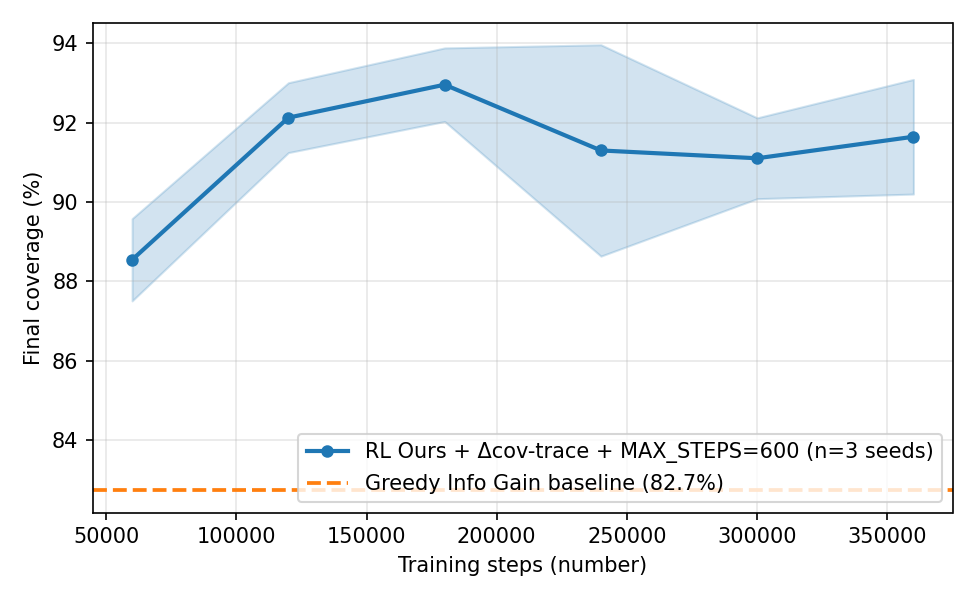
\includegraphics[width=0.325\textwidth]{figures/training_curve_coverage.png}\hfill
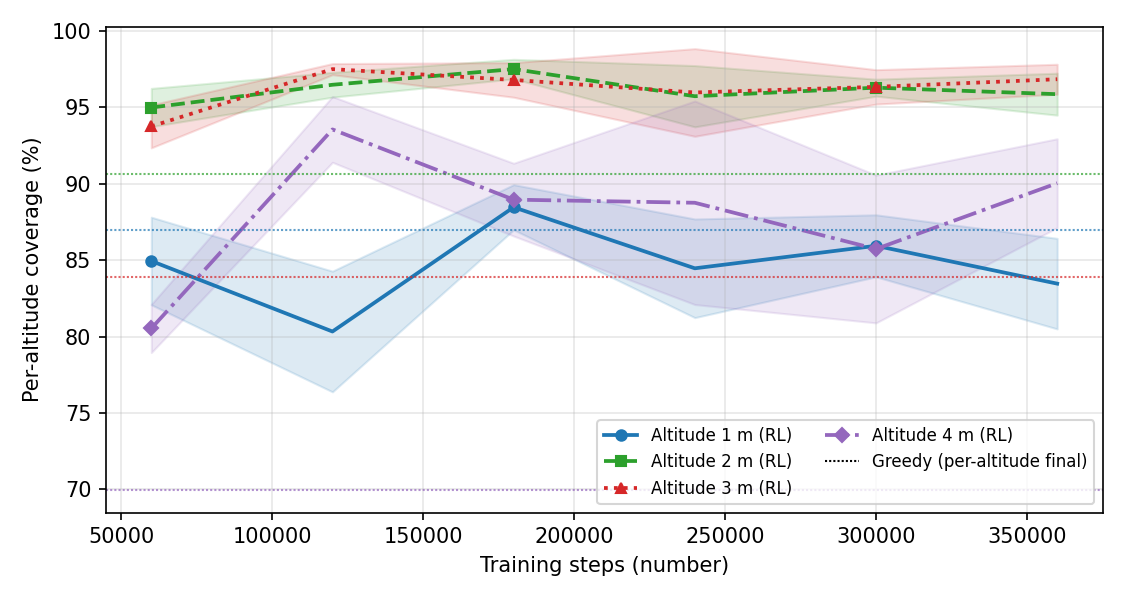
\includegraphics[width=0.325\textwidth]{figures/training_curve_per_altitude.png}\hfill
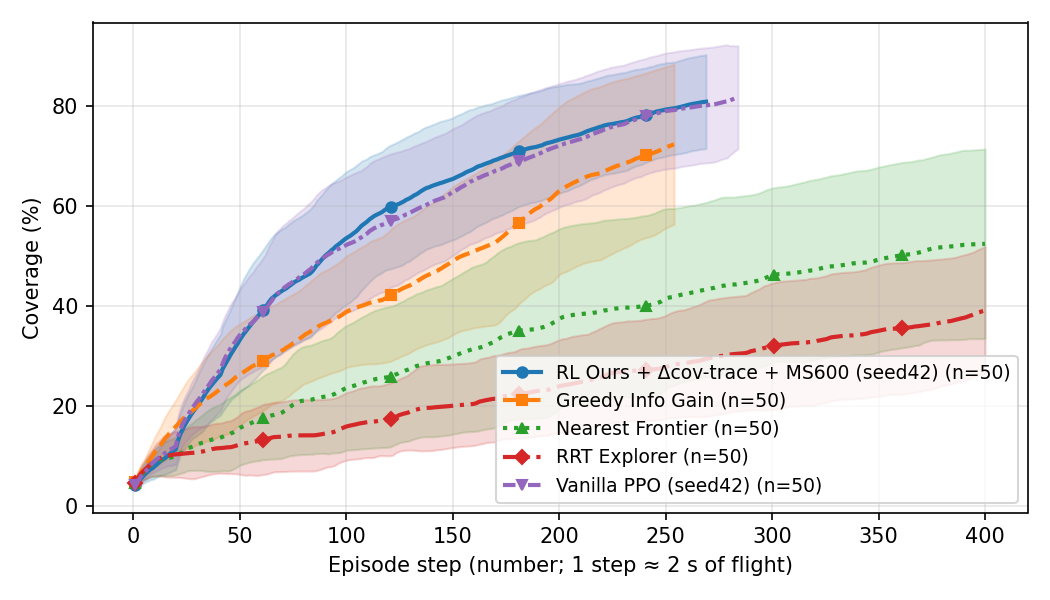
\includegraphics[width=0.325\textwidth]{figures/timeseries_coverage.png}
\caption{(a) Coverage vs.\ training steps (mean $\pm$ std, 3 seeds; dashed: Greedy Info Gain reference). (b) Per-altitude learning curves (solid: RL; dotted: Greedy final altitude coverage). (c) Intra-episode coverage vs.\ step over 50 held-out episodes; RL reaches $50\%$ at step $\sim\!180$, $\sim\!2{\times}$ faster than Greedy.}
\label{fig:curves}
\end{figure}

Fig.~\ref{fig:curves}(a) shows that training coverage rises monotonically and exceeds the Greedy baseline by step $120{,}000$. Fig.~\ref{fig:curves}(b) reveals the multi-altitude strategy: the policy saturates the middle layers (Alt1, Alt2, where shelf content is densest) first, then brings the boundary layers (Alt0, Alt3) above $85\%$, a regime no classical baseline reaches. Fig.~\ref{fig:curves}(c) shows per-step coverage across 50 evaluation episodes: the RL policy is both more thorough (higher final coverage) and faster per unit time, reaching the $50\%$-coverage milestone at step $\sim\!180$ (RL) vs.\ $\sim\!370$ (Greedy) vs.\ $\sim\!580$ (Nearest Frontier).

\subsubsection{Qualitative Multi-Altitude Trajectory}

\begin{figure}[tb]
\centering
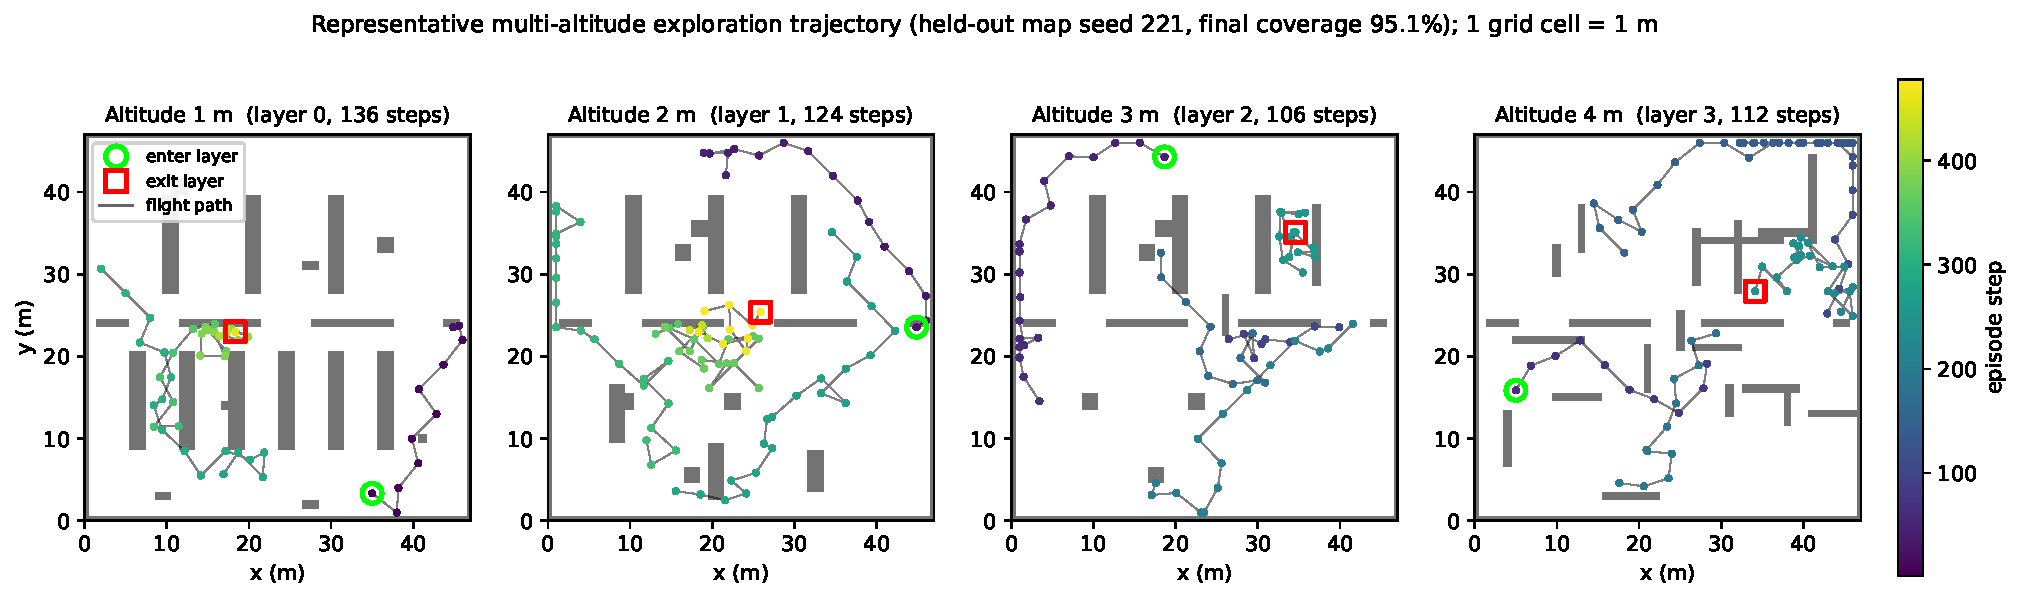
\includegraphics[width=0.86\textwidth]{figures/trajectory_altitudes.pdf}
\caption{Representative learned trajectory on a held-out map (seed 221; final coverage $95.1\%$; one grid cell $=1$\,m). Each panel is one altitude layer, showing obstacles (grey) and the agent's flight path while at that layer, colour-coded by episode step, with enter (circle) and exit (square) markers. The policy allocates comparable effort to all four layers.}
\label{fig:traj}
\end{figure}

Fig.~\ref{fig:traj} visualizes a representative rollout across the four altitude layers. The policy distributes its dwell almost evenly across layers (136, 124, 106, and 112 steps) while reaching $95.1\%$ coverage: each layer is swept densely, the policy then changes altitude (respecting the dwell rule), and revisits near previously mapped regions generate the loop closures that keep $\sigma_t$ bounded, in contrast to classical planners, which collapse onto the boundary layers (Table~\ref{tab:main}).

\subsubsection{Ablation Analysis}
Two ablations are run on the \emph{base} recipe ($T_{\max}\!=\!400$, no $\Delta\sigma$ shaping; mean coverage $87.56\!\pm\!2.45\%$) across the same three seeds.
\textbf{No LoopClosure ($89.41\!\pm\!2.31\%$):} mean coverage is statistically indistinguishable from base ($\Delta\!=\!{+}1.85$ pts), but $\sigma_T$ rises from $3.71$ to $3.82$, confirming that loop closure primarily reduces localization uncertainty rather than improving coverage.
\textbf{No BreadthBonus ($86.54\!\pm\!1.49\%$, $-1.02$ pts vs.\ base):} the mean drop understates the effect; cross-seed standard deviations on Alt0 and Alt3 jump from $4.97\%$ and $4.83\%$ to $9.85\%$ and $9.38\%$, showing that the breadth bonus \emph{stabilizes} per-altitude allocation across seeds rather than raising the mean.
Together with the $+3.21$-pt MS600 horizon extension, these components account for the full $91.90\%$ headline.

%==================================================================
\section{Computational Cost and Real-Time Feasibility}
A policy intended for onboard UAV deployment must fit a companion computer's compute and latency budget. The network has $2{,}023{,}035$ trainable parameters ($\approx\!2.02$\,M) and requires $10.16$\,M multiply--accumulate operations ($20.32$\,M FLOPs) per inference, occupying $\approx\!8$\,MB at single precision, well within embedded-class memory. Measured on a single thread (\texttt{OMP}/\texttt{MKL} pinned) of an Intel Core i5-12450H with no GPU, emulating a UAV companion computer, the forward pass completes in $1.20$\,ms on average ($1.55$\,ms at the $99$th percentile, $\sim\!836$\,Hz), and the full control step including observation construction takes $1.98$\,ms ($\sim\!506$\,Hz). Even a conservative $10\text{--}20\times$ slowdown on an ARM-class processor sustains $25\text{--}80$\,Hz, far above the $\sim\!0.5$\,Hz waypoint-decision rate. Inference is therefore not a deployment bottleneck; the binding real-time constraint is the SLAM backend, discussed next.

%==================================================================
\section{Sim-to-Real Transfer: Findings and Roadmap}\label{sec:sim2real}
The lightweight grid environment mirrors a high-fidelity simulation stack to ease eventual hardware transfer. A companion Gazebo/PX4 software-in-the-loop simulation hosts an \texttt{x500} quadrotor with a $360^\circ$ 2D LiDAR and an RGB-D camera, and RTAB-Map performs real-time visual SLAM, producing the occupancy grid, covariance, and loop closures the environment abstracts. Because the observation and action interfaces match the training environment exactly (a five-channel $48\!\times\!48$ map tensor, a ten-dimensional scalar vector, and a three-dimensional action), the trained checkpoint runs \emph{zero-shot} in Gazebo without fine-tuning. A reactive safety layer (LiDAR/depth avoidance with a covariance-triggered retreat) and a three-tier diagnostic are operational; in an altitude-capped 300-step run the policy explores with stable odometry and zero tracking-loss events, validating the end-to-end pipeline on a real SLAM backend.

The dominant gap between the abstract grid and physical SLAM is motion smoothness: RTAB-Map's visual odometry requires smooth motion, and abrupt reversals, which the grid agent can issue freely because it teleports between cells, degrade tracking and can cascade into pose drift. The deployed, no-retraining mitigation is a per-axis exponential-moving-average action filter that preserves sustained sweeps while damping jitter. Building on this, the environment exposes three transfer-oriented controls (disabled in the experiments above, so the reported results are unaffected): a motion-smoothness reward $-w_{\text{sm}}\|a_t-a_{t-1}\|^2$ that reduces reliance on inference-time filtering, an altitude-transition penalty that discourages the Z-filter thrashing which stalls RTAB-Map re-slicing, and a frontier definition aligned to the RTAB-Map projection. Further milestones include altitude-dependent feature-density modelling, larger geometries, and on-board flight tests. Because the policy already optimizes a localization-uncertainty surrogate, it is predisposed toward the loop-closure-seeking behaviour that real SLAM backends reward.

%==================================================================
\section{Conclusion and Future Work}
We presented a Recurrent PPO approach to multi altitude UAV active SLAM, in which a CoordConv--LSTM actor-critic jointly controls horizontal motion and altitude selection. A fifteen term composite reward, including a novel $\Delta\sigma$ uncertainty-shaping term, a per-altitude breadth bonus, and breadth weighted terminal credit, produces policies reaching $91.90\!\pm\!1.72\%$ coverage across three seeds and fifty held-out maps, dominating all baselines by large effect sizes (Cliff's $\delta\!\geq\!0.49$; Table~\ref{tab:stat}). Ablations confirm the breadth bonus stabilizes per-altitude allocation and the loop closure reward primarily reduces localization uncertainty. Future work will scale to larger geometries, fold a real RTAB-Map backend into the training loop, and pursue physical UAV deployment following the roadmap of Section~\ref{sec:sim2real}.

%==================================================================
%% Bibliography inlined and ordered by first appearance in the text (per the
%% conference instruction), retaining the Springer LNCS (splncs04) entry format and DOIs.
\begin{thebibliography}{18}
\fontsize{7.6}{8.6}\selectfont
\setlength{\itemsep}{0.5pt}
\providecommand{\url}[1]{\texttt{#1}}
\providecommand{\urlprefix}{URL }
\providecommand{\doi}[1]{https://doi.org/#1}

\bibitem{qin2019autonomous}
Qin, H., Meng, Z., Meng, W., Chen, X., Sun, H., Lin, F., Ang, M.H.: Autonomous
  exploration and mapping system using heterogeneous uavs and ugvs in
  gps-denied environments. IEEE Transactions on Vehicular Technology
  \textbf{68}(2),  1339--1350 (2019). \doi{10.1109/TVT.2018.2890416}

\bibitem{zhang2026adaptive}
Zhang, Y., Tan, Z., Liu, K., Yang, Y., Yang, W., Wang, S., Wen, C.Y.: Adaptive
  clustering convexification mapping-planning system for uavs in unknown
  environments. IEEE Transactions on Automation Science and Engineering
  \textbf{23},  5852--5868 (2026). \doi{10.1109/TASE.2026.3670813}

\bibitem{placed2023survey}
Placed, J.A., Strader, J., Carrillo, H., Atanasov, N., Indelman, V., Carlone,
  L., Castellanos, J.A.: A survey on active simultaneous localization and
  mapping: State of the art and new frontiers. IEEE Transactions on Robotics
  \textbf{39}(3),  1686--1705 (2023). \doi{10.1109/TRO.2023.3248510}

\bibitem{zhang2026u}
Zhang, J., Qian, H., Wang, Y., Liang, C., Song, A.: U-slam: Ultrasonic
  simultaneous localization and mapping for underwater pipeline defect
  inspection. IEEE Transactions on Instrumentation and Measurement
  \textbf{75},  1--14 (2026). \doi{10.1109/TIM.2026.3674248}

\bibitem{yin2025maslam}
Yin, Y., Qi, Y., Feng, D., Chen, H., Ma, H., Wu, J., Jiang, Y.: {MA-SLAM}:
  Active {SLAM} in large-scale unknown environment using map aware deep
  reinforcement learning. arXiv preprint arXiv:2511.14330  (2025).
  \doi{10.48550/arXiv.2511.14330}

\bibitem{chen2024lidar}
Chen, J., Wu, K., Hu, M., Suganthan, P.N., Makur, A.: {LiDAR}-based end-to-end
  active {SLAM} using deep reinforcement learning in large-scale environments.
  IEEE Transactions on Vehicular Technology  \textbf{73}(10),  14187--14200
  (2024). \doi{10.1109/TVT.2024.3405483}

\bibitem{zhao2024ddpg}
Zhao, S., Hwang, S.H.: Exploration- and exploitation-driven deep deterministic
  policy gradient for active {SLAM} in unknown indoor environments. Electronics
   \textbf{13}(5), ~999 (2024). \doi{10.3390/electronics13050999}

\bibitem{xu2025navrl}
Xu, Z., Han, X., Shen, H., Jin, H., Shimada, K.: {NavRL}: Learning safe flight
  in dynamic environments. IEEE Robotics and Automation Letters
  \textbf{10}(4),  3668--3675 (2025). \doi{10.1109/LRA.2025.3546069}

\bibitem{asgharivaskasi2023semantic}
Asgharivaskasi, A., Atanasov, N.: Semantic {OcTree} mapping and shannon mutual
  information computation for robot exploration. IEEE Transactions on Robotics
  \textbf{39}(3),  1910--1928 (2023). \doi{10.1109/TRO.2023.3245986}

\bibitem{asgharivaskasi2025riemannian}
Asgharivaskasi, A., Girke, F., Atanasov, N.: {Riemannian} optimization for
  active mapping with robot teams. IEEE Transactions on Robotics  \textbf{41},
  1077--1097 (2025). \doi{10.1109/TRO.2025.3526295}

\bibitem{ebadi2023extreme}
Ebadi, K., Bernreiter, L., Biggie, H., Catt, G., Chang, Y., Chatterjee, A.,
  Denniston, C.E., Desch{\^e}nes, S.P., Harlow, K., Khattak, S., et~al.:
  Present and future of {SLAM} in extreme environments: The {DARPA} {SubT}
  challenge. IEEE Transactions on Robotics  \textbf{40},  936--959 (2024).
  \doi{10.1109/TRO.2023.3323938}

\bibitem{azpurua2023subterranean}
Azp{\'u}rua, H., Saboia, M., Freitas, G.M., Clark, L., Agha-mohammadi, A.a.,
  Pessin, G., Campos, M.F.M., Macharet, D.G.: A survey on the autonomous
  exploration of confined subterranean spaces: Perspectives from real-world and
  industrial robotic deployments. Robotics and Autonomous Systems
  \textbf{160},  104304 (2023). \doi{10.1016/j.robot.2022.104304}

\bibitem{botteghi2021curiosity}
Botteghi, N., Sirmacek, B., Poel, M., Brune, C., Schulte, R.: Curiosity-driven
  reinforcement learning agent for mapping unknown indoor environments. ISPRS
  Annals of the Photogrammetry, Remote Sensing and Spatial Information Sciences
   \textbf{V-1-2021},  129--136 (2021).
  \doi{10.5194/isprs-annals-V-1-2021-129-2021}

\bibitem{garaffa2023survey}
Garaffa, L.C., Basso, M., Konzen, A.A., de~Freitas, E.P.: Reinforcement
  learning for mobile robotics exploration: A survey. IEEE Transactions on
  Neural Networks and Learning Systems  \textbf{34}(8),  3796--3810 (2023).
  \doi{10.1109/TNNLS.2021.3124466}

\bibitem{wang2024exploration}
Wang, M., Xin, B., Jing, M., Qu, Y.: An exploration-enhanced search algorithm
  for robot indoor source searching. IEEE Transactions on Robotics
  \textbf{40},  4160--4178 (2024). \doi{10.1109/TRO.2024.3454572}

\bibitem{kaufmann2023racing}
Kaufmann, E., Bauersfeld, L., Loquercio, A., M{\"u}ller, M., Koltun, V.,
  Scaramuzza, D.: Champion-level drone racing using deep reinforcement
  learning. Nature  \textbf{620}(7976),  982--987 (2023).
  \doi{10.1038/s41586-023-06419-4}

\bibitem{ni2022recurrent}
Ni, T., Eysenbach, B., Salakhutdinov, R.: Recurrent model-free {RL} can be a
  strong baseline for many {POMDPs}. In: Proceedings of the 39th International
  Conference on Machine Learning (ICML). Proceedings of Machine Learning
  Research, vol.~162, pp. 16691--16723. PMLR (2022)

\bibitem{raffin2021sb3}
Raffin, A., Hill, A., Gleave, A., Kanervisto, A., Ernestus, M., Dormann, N.:
  {Stable-Baselines3}: Reliable reinforcement learning implementations. Journal
  of Machine Learning Research  \textbf{22}(268), ~1--8 (2021)

\end{thebibliography}

\end{document}